\documentclass[10pt,twoside]{article}

\usepackage[margin=1in]{geometry}
\usepackage{epsfig}
\usepackage{calc}
\usepackage{amssymb}
\usepackage{amstext}
\usepackage{amsmath}
\usepackage{amsthm}
\usepackage{multicol}
\usepackage{pslatex}
\usepackage{apalike}
\usepackage{graphicx}
\usepackage{caption}
\usepackage{subcaption}

\begin{document}

\title{6.867 Machine Learning  \subtitle{Homework 2} }

\maketitle

% **************************************************************************************************
 % Problem 1
% **************************************************************************************************

\section{\uppercase{Logistic Regression}}

\noindent Logistic Regression is a discriminative model used for classification. Given an input $x$, it finds the posterior of $x$ belonging to one of the classes and then uses that probability to classify $x$. In the simplest case, it takes a linear combination of the input $x$ and uses that as an input to the sigmoid function, which outputs a number between 0 and 1. The sigmoid function is shown below. 

\begin{equation}
\sigma(x) = \frac{1}{1+e^{-x}}
\end{equation}

One of the problems with logistic regressions is that they are very prone to overfitting to the training data. One way to prevent the overfitting is to add a regularization term, $\lambda$, which penalizes the size of the weight vector. The size of the weight vector can be penalized using the $L_1$ norm and the $L_2$ norm. Here, we explore how different values of $\lambda$  and the different norms affect several aspects of the logistic regression. The objective function for logistic regression and its gradient are shown below. 

\begin{equation}
NLL(w,w_0) = \sum_i \log(1+exp(-y^{(i)}(wx^{(i)}+w_0))) + \lambda \left \| w \right \|_2^2
\end{equation}

\begin{equation}
\nabla NLL(W) = \sum_{i=1}^n (\sigma (W^Tx^{(i)})-y^{(i)})x^{(i)} + 2\lambda 
\end{equation}

with $W = (w,w_0)$



\subsection{Optimizing with Gradient Descent}

\noindent To investigate how $L_2$ regularization affected the logistic regression we tried $\lambda = 0$ and $\lambda = 1$. We decided not to penalize the bias term in the weight vector. We found that with $\lambda = 1$ the weight vector decreased in every iteration of the algorithm until it converged to its optimal value. We believe this is because for most iterations, the quickest way to decrease the objective function is to decrease the norm of the weight vector, because it is penalized by a quadratic factor. With $\lambda = 0$, the opposite happened. The norm of the weight increased in every iteration until it converged to its optimal value. Unregularized logistic regressions attempt to make the weight vector as large as possible because that makes the sigmoid function steeper, which in turn increases the log likelihood of the data. Our obersvations agree with our intuition that regularization makes the weight vector smaller.

\begin{figure}[h]
        \begin{subfigure}[b]{0.5\textwidth}
                \centering
                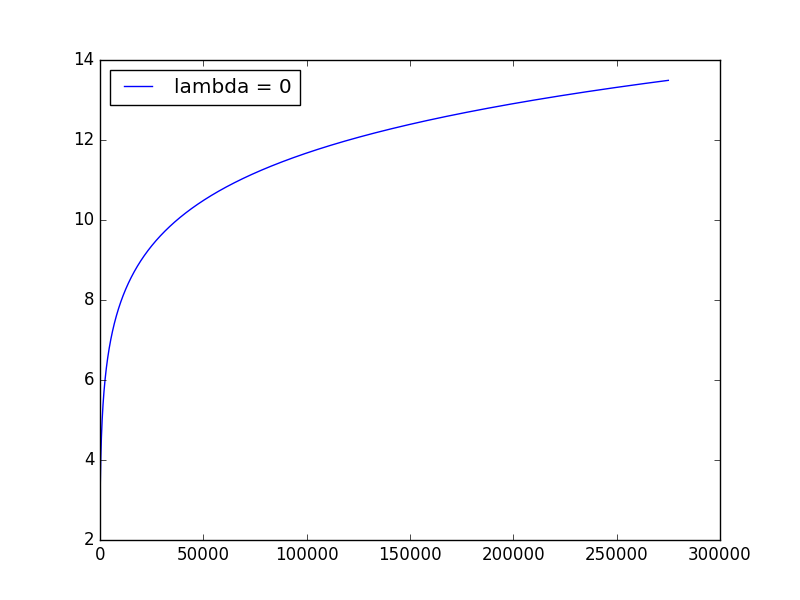
\includegraphics[width=\linewidth]{Figures/P1/1_1_L0.png}
                \caption{Graph of Norm of weight vector with lmbda = 0}
        \end{subfigure}%
        \begin{subfigure}[b]{0.5\textwidth}
                \centering
                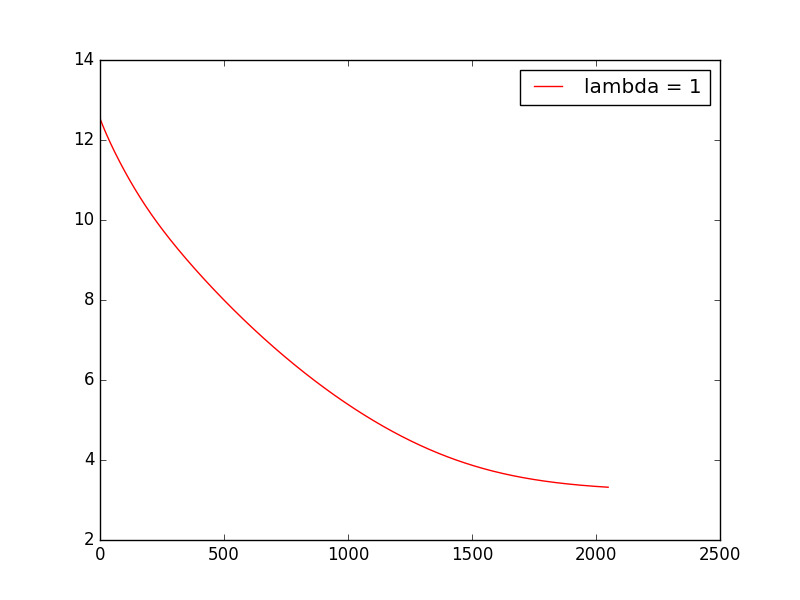
\includegraphics[width=\linewidth]{Figures/P1/1_1_L1.png}
                \caption{Graph of Norm of weight vector with lmbda = 0}
        \end{subfigure}
        \caption{Pictures of animals}
\end{figure}

\subsection{Section1??}


You should be able to concisely represent trends for those configurations. For example, you could have one plot showing the effect of the error rate for different regularizers and lambdas, a good example of changing the decision boundary, and general observations, and maybe a plot about the weights. Perform your experiments and see what makes the most sense.

\subsection{L1 vs L2 Norm}

Two common metrics used to penalize the size of the weight vector are the $L_1$ and $L_2$ norm. The norms are defined as follows: ($L_1$ is sum of absolute values). We tested the effect of each of these norms and different lambda values on the Classification Error Rate, decision boundary, and the weights of the weight vector. We used scikit-learn's implementation of Logistic Regression, which also penalizes the bias term. To allow for unpenalized bias, the logistic regression has an additional parameter, intercept_scaling, which is a factor by which the intercept is multiplied by to offset the effects of the regularization. We set the value of the intercept scaling to be equal to the lambda value. We tested both the $L_1$ and $L_2$ model with lambda values ranging from $10^{-5}$ to $10^5$. 

Effect on Classification Error Rate:
In general, we found that the regularization seemed to have a larger effect on the CER when using the $L_1$ norm then when using the $L_2$ norm. The $L_2$ norm logistic regression was able to maintain low CER's even with high lambda values. The $L_1$ norm, on the other hand, often drove the weight vector to zero, which increased the CER. For most data sets, the $L_2$ norm achieved a better CER than the $L_1$ norm when set to the same lambda values. When both weight vectors were nonzero, their CER's usually only differed by a percentage point. The difference between the CER's grew dramatically whenever the $L_1$ norm drove one of the weights in the weight vector to zero. The two models generally behaved that way except for the last data set, in which the data was linearly inseparable. There, the $L_1$ and $L_2$ norm achieved very similar CER scores for every lambda value we tested. 

\begin{figure}[h]
        \begin{subfigure}[b]{0.5\textwidth}
                \centering
                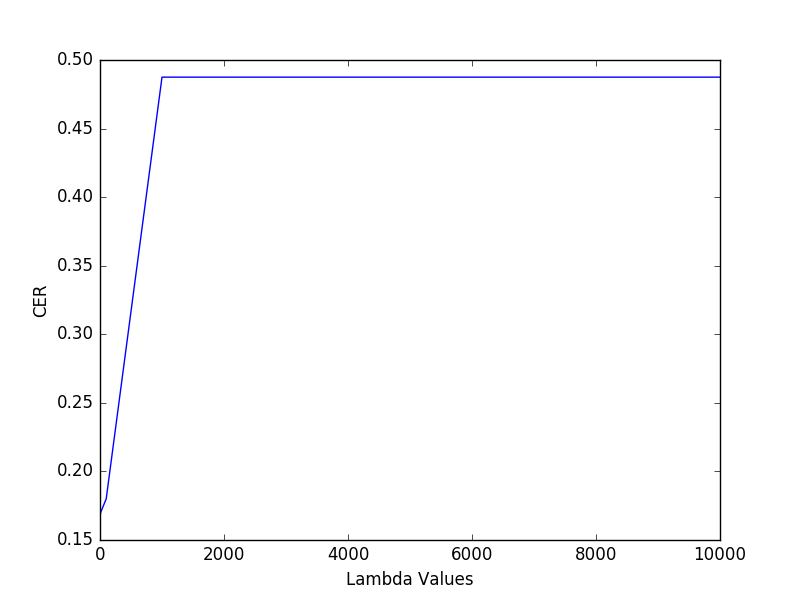
\includegraphics[width=\linewidth]{Figures/P1/B_CERL1.png}
                \caption{Classification Error Rate of $L_1$ norm as a function of Lambda}
        \end{subfigure}%
        \begin{subfigure}[b]{0.5\textwidth}
                \centering
                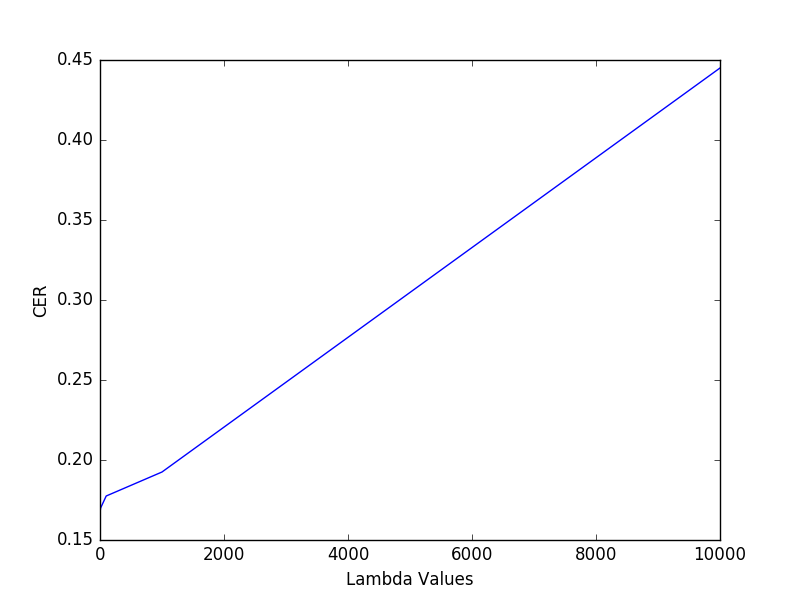
\includegraphics[width=\linewidth]{Figures/P1/B_CERL2.png}
                \caption{Classification Error Rate of $L_2$ norm as a function of Lambda}
        \end{subfigure}
        \caption{Pictures of animals}
\end{figure}

Effect on Decision Boundary 
As mentioned in the previous section, the $L_1$ norm tends to drive the weights of the weight vector to zero as lambda increases. As a result, there were several instances where the decision boundary was simply the x axis CHECK THIS. In general, we found that decreasing lambda changed the decision boundary in a direction where it could better separate the training data. This was true for all of the data sets where the data was linearly separable. For the data set in which the data was linearly inseparable, the decision boundary never changed, regardless of the lambda value. 

\begin{figure}[h]
        \begin{subfigure}[b]{0.25\textwidth}
                \centering
                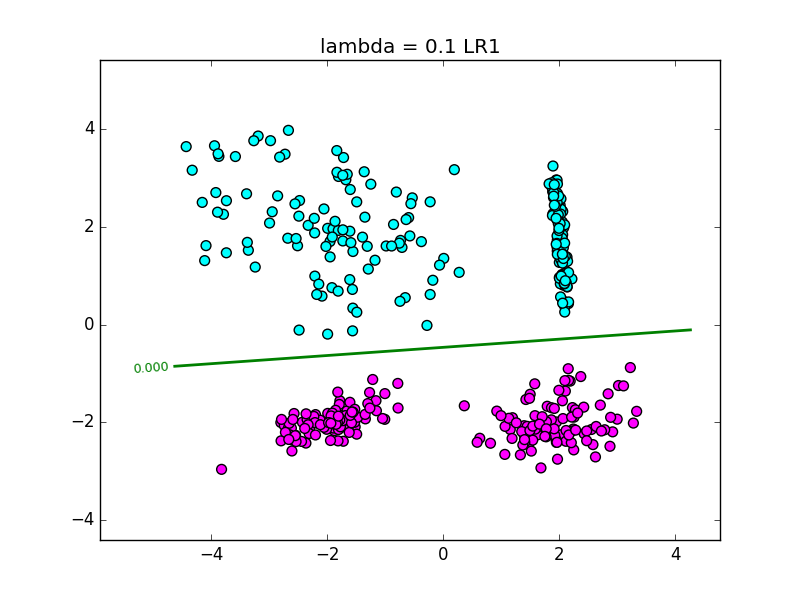
\includegraphics[width=\linewidth]{Figures/P1/LR1__1.png}
                \caption{$\lambda = 0.1$}
                \label{fig:gull}
        \end{subfigure}%
        \begin{subfigure}[b]{0.25\textwidth}
                \centering
                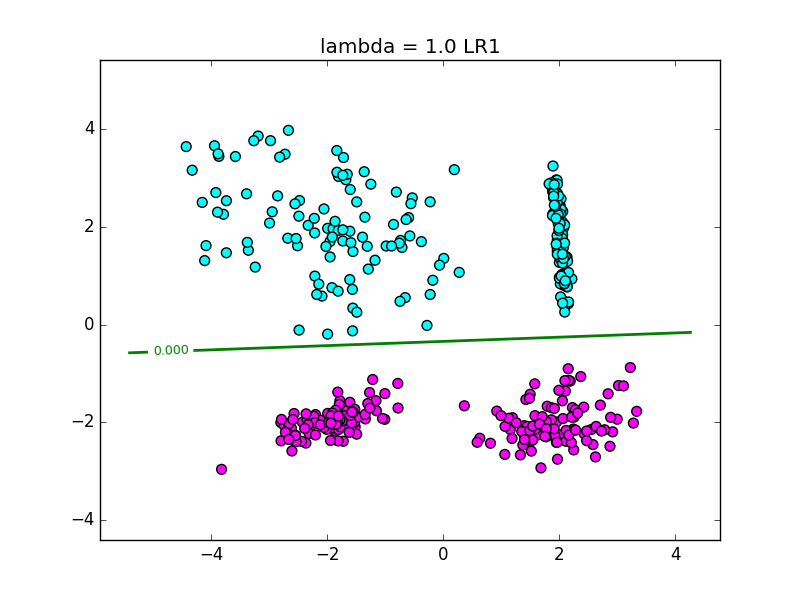
\includegraphics[width=\linewidth]{Figures/P1/LR1_1.png}
                \caption{$\lambda = 1$}
                \label{fig:gull2}
        \end{subfigure}%
        \begin{subfigure}[b]{0.25\textwidth}
                \centering
                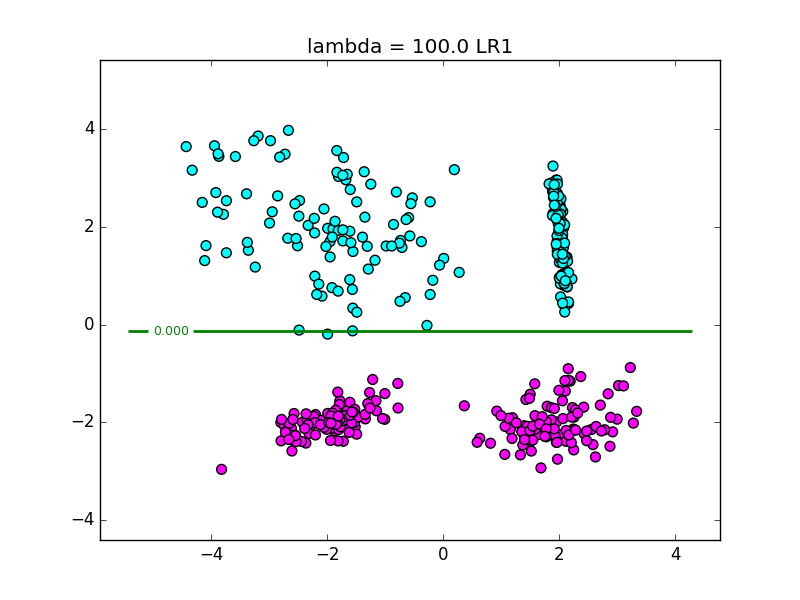
\includegraphics[width=\linewidth]{Figures/P1/LR1_100.png}
                \caption{$\lambda = 100$}
                \label{fig:tiger}
        \end{subfigure}%
        \begin{subfigure}[b]{0.25\textwidth}
                \centering
                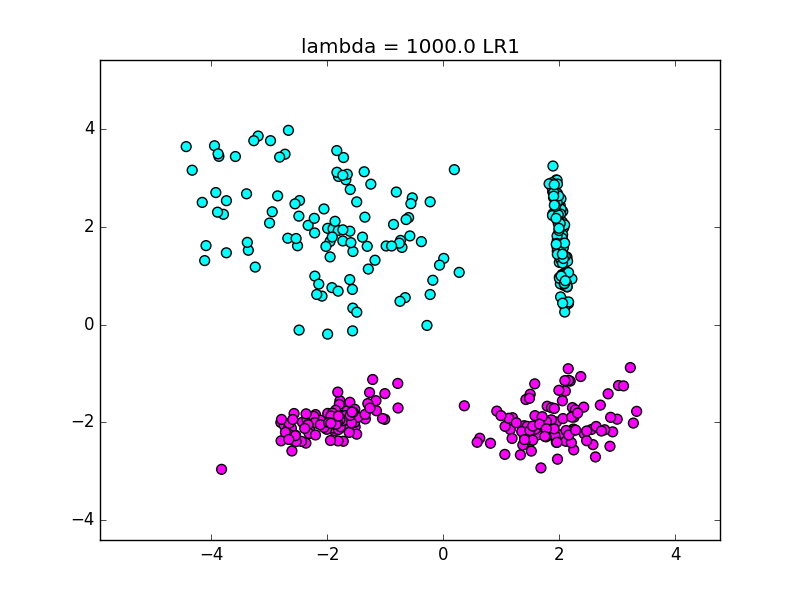
\includegraphics[width=\linewidth]{Figures/P1/LR1_1000.png}
                \caption{$\lambda = 1000$}
                \label{fig:mouse}
        \end{subfigure}
        \caption{$L_1$ Regularization with different $\lambda$s}\label{fig:animals}
\end{figure}


Effect on Weights
Higher lambda values decreased the weights of the weight vector in both models. Higher lambda values affected the $L_1$ model a lot more, as it was more likely to have zero valued weights. The $L_2$ model was more likely to have very small, but still nonzero weights. 

\subsection{Optimal Parameters}
We evaluated the performance of both norms on different data sets using the same lambda values as before. We found that when using $L_1$ regularization, a lambda value of 0.1 achieved the best performance on both the validation and the test sets. With $L_2$ regularization the optimal value for lambda was 1. Both of these values can be modified by a factor of 10 without significantly hurting the accuracy. With these values, the two models achieved nearly identical results on all data sets, the difference in performance was never more than half a percentage point.

\subsection{Section2}



% **************************************************************************************************
 % Problem 2
% **************************************************************************************************

\section{\uppercase{Support Vector Machines}}

Support Vector Machines are supervised learning models that work by finding a dividing hyperplane between the training data while maximizing the gap between the training data and the decision boundary. This is to help the classifier generalize better and makes it more robust to noise. Assuming the data is linearly separable, finding this dividing hyperplane amounts to solving the quadratic program

\begin{equation}
\begin{array}{ll@{}ll}
\text{min}  & \displaystyle \frac{1}{2} ||w||^2 &\\
\text{s. t.}& \displaystyle y^i(w^T x^i + b) \geq 1 , 1 \leq i \leq n
\end{array}
\end{equation}

where $w$ is the vector perpendicular to the dividing hyperplane and $\frac{1}{||w||}$ is the size of the margin.

If the data is almost but not completely linearly separable, we can still model the data with an SVM by introducing slack variables when solving for a classifier. We allow the training points to be misclassified by some amount $e$ and the goal is to maximize the margin while minimizing the slack. This formulation is called C-SVM and the separating hyperplane can be found by solving the quadratic program below.

\begin{equation}
\begin{array}{ll@{}ll}
\text{min}  & \displaystyle \frac{1}{2} ||w||^2 + C \sum_i e_i &\\
\text{s. t.}& \displaystyle y^i(w^T x^i + b) \geq 1 - e_i , 1 \leq i \leq n \\
& e_i \geq 0 , 1 \leq i \leq n
\end{array}
\end{equation}

\subsection{Dual Formulation of C-SVM}
This problem as stated above is difficult to implement with kernels functions. Fortunately, we convert the problem from the primal formulation stated above and instead implement its dual formuation.

\begin{equation}
\begin{array}{ll@{}ll}
\text{min}  & \displaystyle \frac{1}{2} \sum_{i=1}^{n} \sum_{j=1}^n \alpha_i \alpha_j y_i y_j [\phi(x_i)^T \phi(x_j)] - \sum_{t=1}^{n} \alpha_t &\\
\text{s. t.}& \displaystyle 0 \leq a_t \leq C , \sum_{t=1}^{n} \alpha_t y_t = 0
\end{array}
\end{equation}

To solve this linear program and get the $\alpha$s, we used the solver in a python library called cvxopt. The solver finds solutions to quadratic programs of the form:

\begin{equation}
\begin{array}{ll@{}ll}
\text{min}  & \displaystyle \frac{1}{2} x^T P x + q^T x &\\
\text{s. t.}& \displaystyle G x \leq h &\\
& Ax = b
\end{array}
\end{equation}

In our case, our matrices are 

\begin{equation*}
P = Diag(\overrightarrow{y}) X X^T Diag(\overrightarrow{y})
\end{equation*}
\begin{equation*}
q = -1 * \overrightarrow{1}
\end{equation*}
\begin{equation*}
G = [I | -I]
\end{equation*}
\begin{equation*}
h = [C * \overrightarrow{1} | \overrightarrow{0}]
\end{equation*}
\begin{equation*}
A = \overrightarrow{y}
\end{equation*}
\begin{equation*}
b = 0
\end{equation*}

$Diag(\overrightarrow{y})$ is a diagonal matrix with $y^{(i)}$s on the diagonal.

This solver returns $\overrightarrow{x}$ which is our $\overrightarrow{\alpha}$ vector.

Testing this implementation, we created a dataset with four points. The positive examples were $(2, 2),(2, 3)$ and the negative examples where $(0, -1),(-3, -2)$. The solver returned
\begin{equation}
\overrightarrow{\alpha} = [1.54e-01, 7.02e-08, 1.54e-01, 9.15e-09]
\end{equation}

Notice how $\alpha_1$ and $\alpha_3$ are much larger than the rest. This means that these two are the support vectors and they correspond to points $(2,2)$ and $(0,-1)$. The graph of the decision boundary for this small example is shown in figure ? and the support vectors are the points predicted.

\begin{figure}[h]
    \centering
    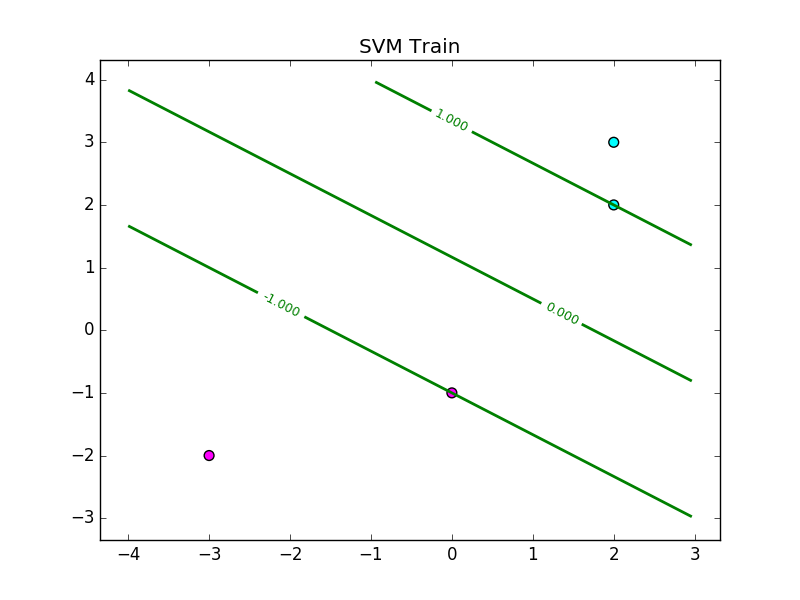
\includegraphics[width=60 mm]{Figures/P2/dumb.png}
    \caption{SVM with linear kernel on four data points. }
\end{figure}



\subsection{2D Dataset Results}

We used our implementation of SVM to classify 2D points and generated plots of the decision boundary and the margins. Figure ? shows SVM run on four different training sets with linear kernels and a slack penalty, $C$, of 1. It is clear the datasets 1 and 3 are meant to be separated by a linear function while datasets 2 and 4 are not. Thus only the separating decision boundary for 1 and 3 are reasonable. The table below shows the training, validation, and test classification error rates. Unsurprisingly, datasets 2 and 4 have terrible classifications rates.

\begin{figure}
        \begin{subfigure}[b]{0.25\textwidth}
                \centering
                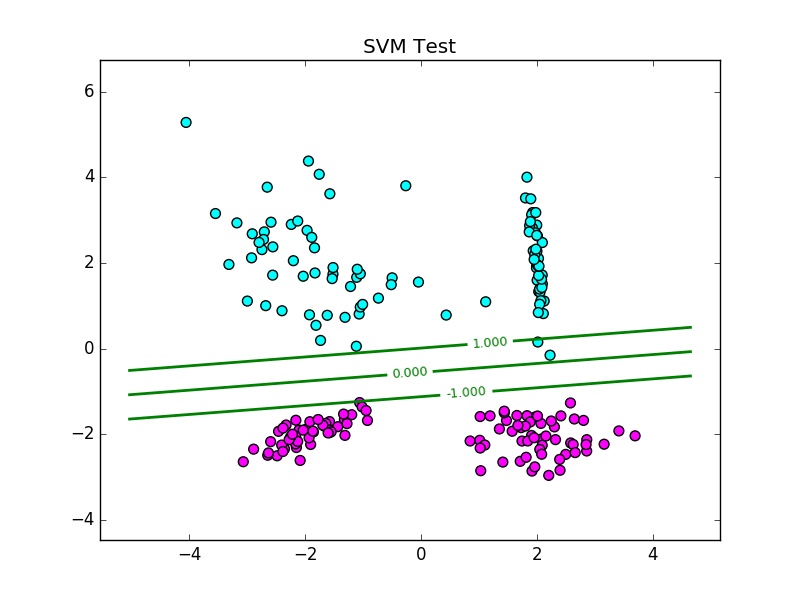
\includegraphics[width=\linewidth]{Figures/P2/svm_data1_test_C1.png}
                \caption{Dataset 1, C=1}
        \end{subfigure}%
        \begin{subfigure}[b]{0.25\textwidth}
                \centering
                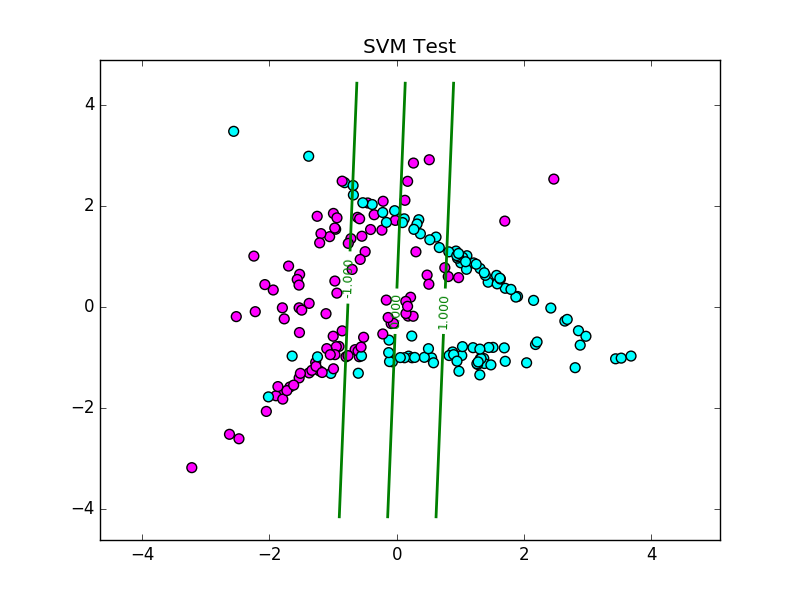
\includegraphics[width=\linewidth]{Figures/P2/svm_data2_test_C1.png}
                \caption{Dataset 2, C=1}
        \end{subfigure}%
        \begin{subfigure}[b]{0.25\textwidth}
                \centering
                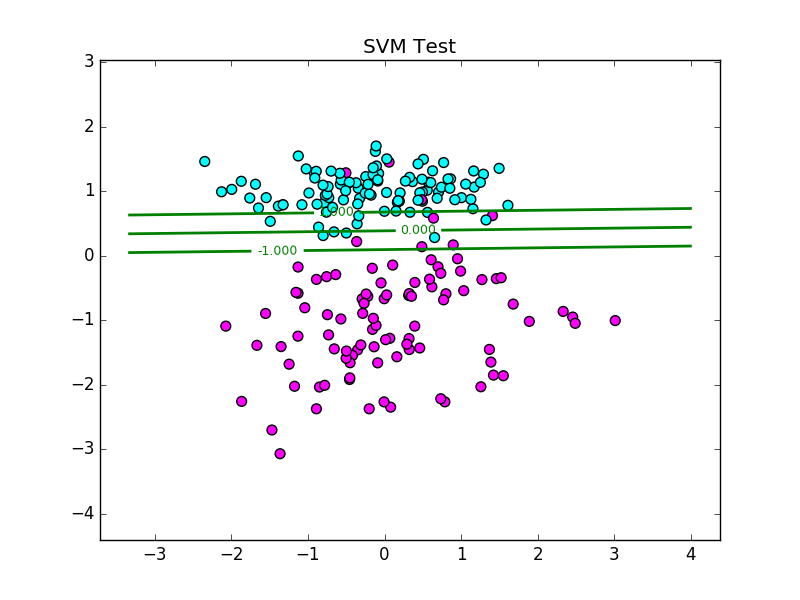
\includegraphics[width=\linewidth]{Figures/P2/svm_data3_test_C1.png}
                \caption{Dataset 3, C=1}
        \end{subfigure}%
        \begin{subfigure}[b]{0.25\textwidth}
                \centering
                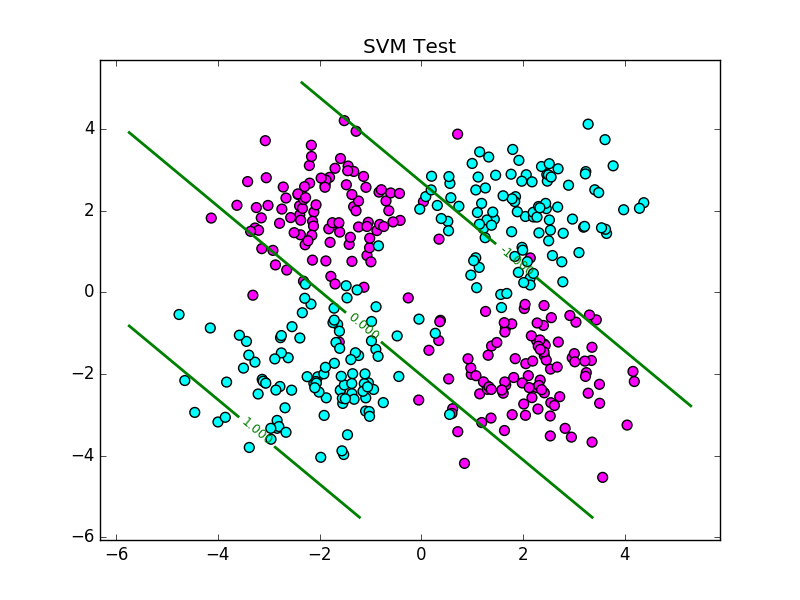
\includegraphics[width=\linewidth]{Figures/P2/svm_data4_test_C1.png}
                \caption{Dataset 4, C=1}
        \end{subfigure}
        \caption{Linear SVM perfomance of different datasets. Datasets 1 and 3 are relatively linearly separable so this SVM performs well on them. Dataset 2 and 4 are definitely not linearly separable so this SVM is not the right model for the data.}\label{fig:animals}
\end{figure}

\begin{center}
 \begin{tabular}{||c c c c||} 
 \hline
  & Training Error & Validation Error & Test Error \\ [0.5ex] 
 \hline\hline
 Dataset 1 & 0 & 0 & 0 \\ 
 \hline
 Dataset 2 & 0.1775 & 0.18 & 0.195 \\
 \hline
 Dataset 3 & 0.02 & 0.03 & 0.045 \\
 \hline
 Dataset 4 & 0.3 & 0.305 & 0.3 \\
 \hline
\end{tabular}
\end{center}

\subsection{2D Dataset Results with Kernel Functions}

Support Vector Machines can still be used to classify not linearly separable data. To do this, we need to either map the data points to higher dimensions or use a nonlinear kernel. To obtain a better classification for dataset 4, we used a Gaussian radial basis function (RBF) kernel with $\gamma = 1$. The result is shown in figure b of figure ? and it achieved a test error rate $4.75\%$.


\subsection{Effect of C on Margin}
The amount of penalty $C$ given to the slack variables can have a large impact on the size of the margin. The small $C$ is, the more the algorithm is willing to give slack to the data points. Thus the size of the margin will increase. As $C$ goes to infinity, the boundary becomes more and more like Hard-SVM. 

This relationship between $C$ and the margin size is true for both linear and nonlinear kernels. In figure ?, the graphs with linear kernels are in order of increasing $C$. We can clearly see the margin is decreasing in size. In figure ?, the graphs with nonlinear kernels also have decreasing margin size with increasing $C$. As the margin decreases, the number of support vectors, that is the number of vectors that are within or on the the margin or the number of points with nonzero $\alpha$s, also decreases. This is clear because less points fall on the wrong side of their margin boundary. Thus as $C$ increases, the number of support vectors decrease. 

When optimizing and choosing a $C$, maximizing the geometric margin should not be the goal. The goal should instead be minimizing the error rate in the validation set. A large geometric margin is not related to a low error rate. In fact, a large geometric margin means lots of support vectors which leads to slow runtimes. 

\begin{figure}[h]
        \begin{subfigure}[b]{0.33\textwidth}
                \centering
                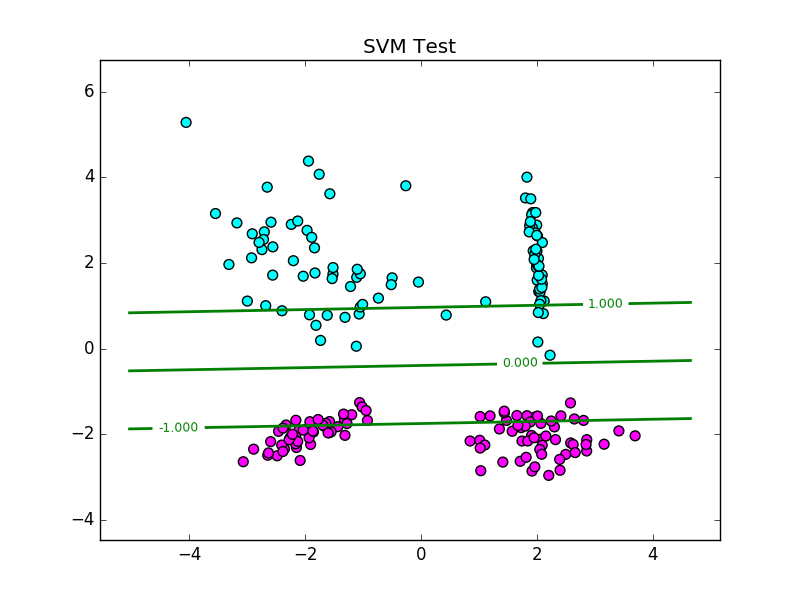
\includegraphics[width=\linewidth]{Figures/P2/svm_data1_test_C-2.png}
                \caption{Dataset 1, C=0.01}
        \end{subfigure}%
        \begin{subfigure}[b]{0.33\textwidth}
                \centering
                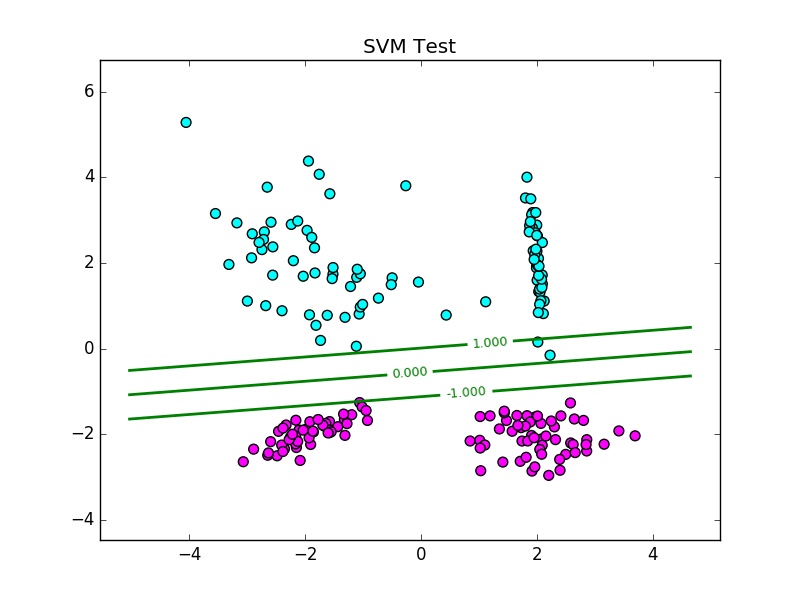
\includegraphics[width=\linewidth]{Figures/P2/svm_data1_test_C1.png}
                \caption{Dataset 1, C=1}
        \end{subfigure}%
        \begin{subfigure}[b]{0.33\textwidth}
                \centering
                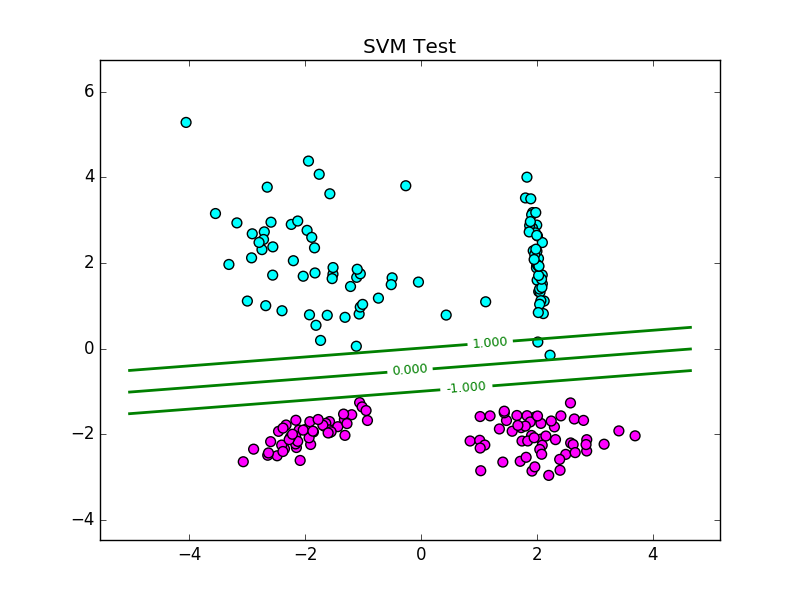
\includegraphics[width=\linewidth]{Figures/P2/svm_data1_test_C100.png}
                \caption{Dataset 1, C=100}
        \end{subfigure}%
        \caption{Decision boundary for SVM with linear kernel. The margin clearly gets smaller for large C}
\end{figure}

\begin{figure}[h]
        \begin{subfigure}[b]{0.33\textwidth}
                \centering
                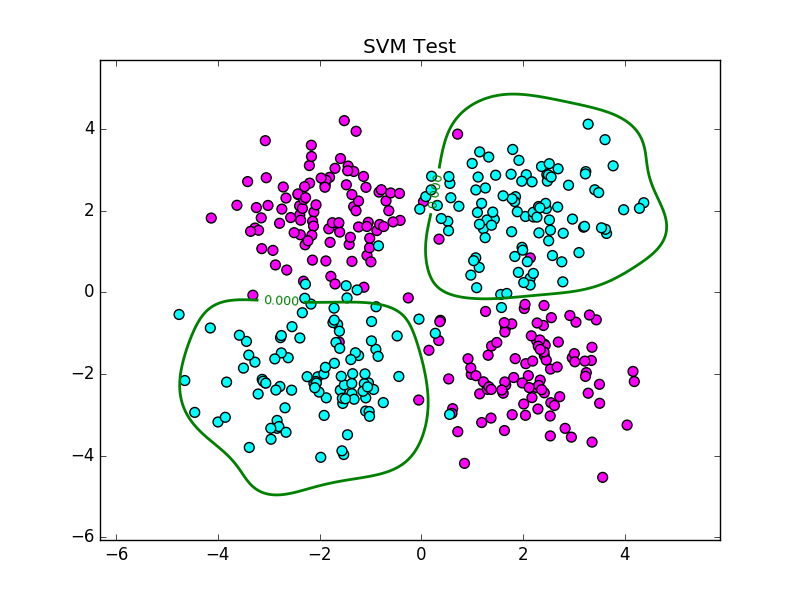
\includegraphics[width=\linewidth]{Figures/P2/RBF_data4_test_g1C-2.png}
                \caption{Dataset 4, C=0.01}
        \end{subfigure}%
        \begin{subfigure}[b]{0.33\textwidth}
                \centering
                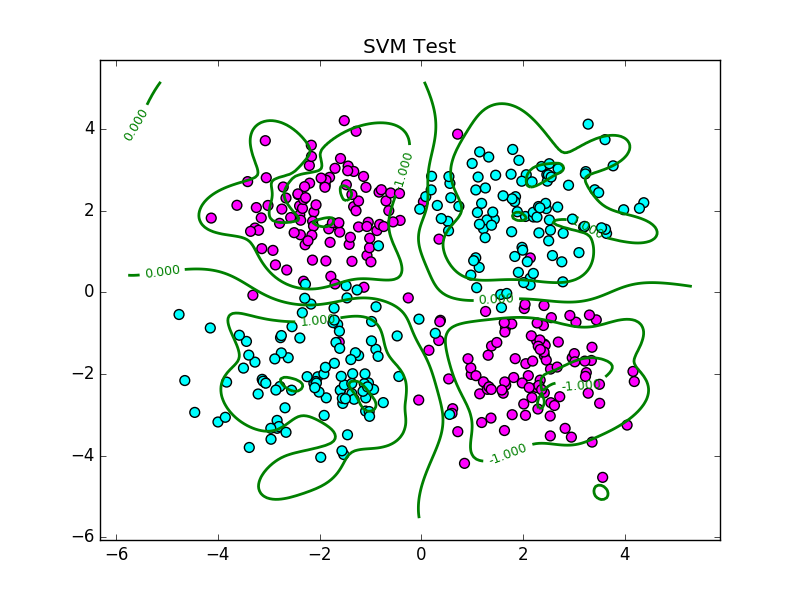
\includegraphics[width=\linewidth]{Figures/P2/RBF_data4_test_g1C1.png}
                \caption{Dataset 4, C=1}
        \end{subfigure}%
        \begin{subfigure}[b]{0.33\textwidth}
                \centering
                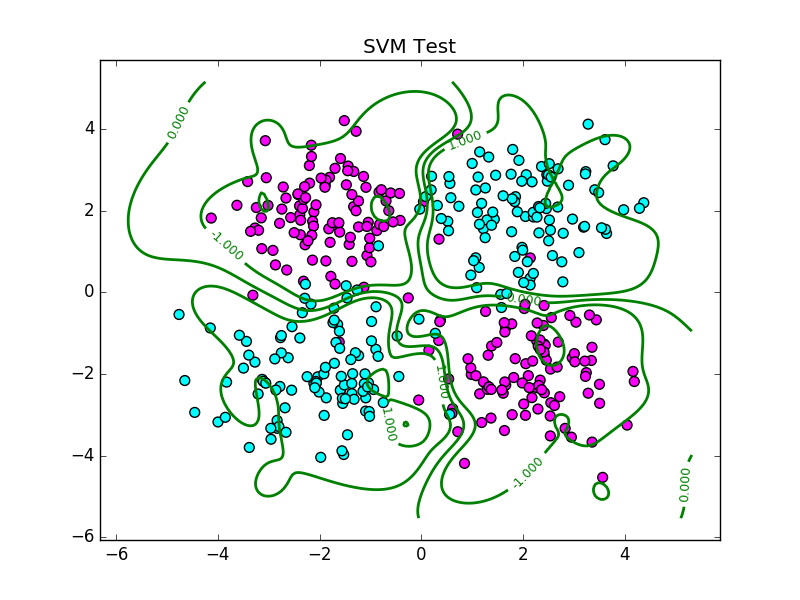
\includegraphics[width=\linewidth]{Figures/P2/RBF_data4_test_g1C100.png}
                \caption{Dataset 4, C=100}
        \end{subfigure}%
        \caption{Decision boundary for SVM with Gaussian RBF kernel. In figure a, the margins are so big they almost do not show up in the graph. By figure c, they have shrunk considerably closer to the decision boundary.}
\end{figure}


% **************************************************************************************************
 % Problem 3
% **************************************************************************************************

\section{\uppercase{Support Vector Machine with Pegasos}}

Even though SVMs have some nice properties, it can be very inefficient to solve large SVMs. One solution for this is the Pegasos algorithm. The Pegasos algorithm is a stochastic gradient descent method that can very quickly find optimal or nearly optimal parameters for an SVM. The Pegasos algorithm can be used to solve the following formulation of the Soft SVM minimization problem. 

\begin{equation}
\min_w \frac{\lambda}{2}\left \| w \right \|^2 + \frac{1}{n} \sum_{i=1}^n \max{0,1-y^{(i)}(w^Tx^{(i))})} 
\end{equation}

This formulation of Soft-SVM is equivalent to C-SVM with $C = \frac{1}{n\lambda}$. The algorithm updates the weight vector for the linear decision boundary of the SVM according to the following update rule if it misclassifies a training sample: 

\begin{equation}
w_{t+1}\leftarrow (1 - \frac{1}{t} )w_t + \frac{1}{t\lambda}y_ix_i
\end{equation}

And it updates it according to this rule if it correctly classifies a training sample:

\begin{equation}
w_{t+1}\leftarrow (1 - \frac{1}{t} )w_t 
\end{equation}

\subsection{Linear SVM}
We implemented the Pegasos algorithm to solve the objective function shown above and tested several values of lambda between 2^1 and 2^-10. We found that the margin shrank as lambda was increased. 


\subsection{Kernelized Pegasos}
The Pegasos algorithm can be easily modified to support Kernels. We implemented this modification and evaluated the performance of SVMs trained using Pegasos. The modification involves finding the actual $\alpha$ values instead of the weights for the linear decision boundary. Having found the optimal $\alpha$s, the decision rule becomes $\sum_j \alpha_j K(x_j,x_i)$. If that sum is positive for a vector $x$, then that sample is classified as positive, otherwise, it is classified as negative. 

Having implemented the Kernelized version of the Pegasos algorithm, we classified the same data as before, but we used a Gaussian kernel. With a fixed value of $\lambda = .02$, we tested out values for $\gamma $ between $2^2$ and $2^{-2}$. We found that as $\gamma $ increased, the number of support vectors also increased. We believe that this is because the increasing $\gamma $ decreases the variance of the guassian kernel. This means that it becomes harder for points to satisfy the constraints 


% **************************************************************************************************
 % Problem 4
% **************************************************************************************************

\section{\uppercase{Handwritten Digit Recognition with MNIST}}
Using the three classification algorithms we developed in this paper, we attempted to classify hand-written digits from the MNIST dataset and compared their performances. Since all the algorithms performed only two-way classification, our goal was to distinguish a certain set of digits for another set of digits. Images of digits from one set were labeled $1$ and while digits from the other set were labeled $-1$.

The training sets used consisted of 200 images of each digit to be classified. Validation and test sets contained 150 for each digit. Each 28 X 28 image was treated as an vector of length 784. We tried the following classfication tasks:  1 vs 7, 3 vs 5, 4 vs 9, (0, 2, 4, 6, 8) vs (1, 3, 5, 7, 9) and also explored the effect of normalizing the image vectors on an algorithm ability to classify the digits. Normalizing a pixel means taking its 0-255 value and mapping it to the range $[-1,1]$. 

The table below shows test error rates for each classification method.

\begin{center}
 \begin{tabular}{||c c c c||} 
 \hline
  & Logistic Regression & Linear SVM & Gaussian RBF SVM & Pegasos \\ [0.5ex] 
 \hline\hline
 1 vs 7 & 0 & 0 & 0 \\ 
 \hline
 3 vs 5 & 0.1775 & 0.18 & 0.195 \\
 \hline
 4 vs 9 3 & 0.02 & 0.03 & 0.045 \\
 \hline
 Even vs Odd 4 & 0.3 & 0.305 & 0.3 \\
 \hline
\end{tabular}
\end{center}

\subsection{Logistic Regression vs Linear SVM}
The classification accuracies of logistic regression and linear SVM for most tasks are very similar. On normalized data, both achieved zero training error on all tasks while getting $95-99\%$ accuracy on test data.
Logistic regression performs the same with or without normalization.

\subsection{Effect of C on Margin}

\vfill
\end{document}

